\documentclass{article}
\usepackage[utf8]{inputenc}
\usepackage{amsmath, amssymb}
\usepackage{graphicx}
\usepackage{hyperref}
\usepackage{tikz}
\usepackage{tikz-cd}
\usepackage{pdfpages}
\usetikzlibrary{matrix, arrows.meta, positioning}

\title{Category Theory Notes}
\author{Yiwen Ding\\
  \texttt{yiwen.ding@example.com}\\% replace with your email
  \textit{Based on note from Oct 10, 2024}}
\date{\today}

\begin{document}

\maketitle

\section{Category Theory}

\subsection{Definition of a Category}

A \textbf{category} consists of:
\begin{itemize}
    \item \textbf{Objects}
    \item \textbf{Morphisms} with domain and codomain
    \item \textbf{Composition} of morphisms
\end{itemize}

\subsection{The Axioms for a Category}

\subsubsection{Associativity}

For composable morphisms $f$, $g$, $h$:
\[
(h \circ g) \circ f = h \circ (g \circ f)
\]

\begin{center}
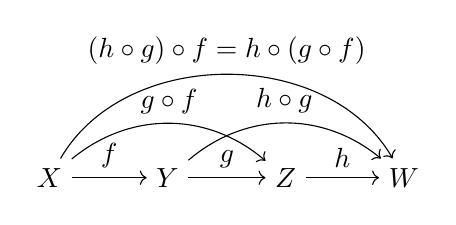
\begin{tikzpicture}[node distance=1.5cm, auto]
  \node (X) {$X$};
  \node (Y) [right of=X] {$Y$};
  \node (Z) [right of=Y] {$Z$};
  \node (W) [right of=Z] {$W$};
  \path[->] (X) edge node {$f$} (Y)
            (Y) edge node {$g$} (Z)
            (Z) edge node {$h$} (W)
            (X) edge[bend left=40] node[above] {$g \circ f$} (Z)
            (Y) edge[bend left=40] node[above] {$h \circ g$} (W)
            (X) edge[bend left=60] node[above] {$(h \circ g) \circ f = h \circ (g \circ f)$} (W);
\end{tikzpicture}
\end{center}

\subsubsection{Identity}

For each object $X$, there exists an identity morphism $1_X : X \to X$ such that for any $f : X \to Y$:
\[
1_X \circ f = f \quad \text{and} \quad f \circ 1_Y = f
\]

\begin{center}
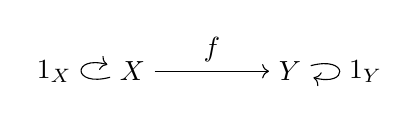
\begin{tikzpicture}[node distance=2cm, auto]
  \node (X) {$X$};
  \node (Y) [right of=X] {$Y$};
  \path[->] (X) edge node {$f$} (Y)
            (X) edge[loop left] node {$1_X$} (X)
            (Y) edge[loop right] node {$1_Y$} (Y);
\end{tikzpicture}
\end{center}

\textbf{Question:} Why is $1_X$ unique?

\textbf{Proof:} Assume there exist $1_X$ and $1_X'$ such that for all $f : X \to Y$ we have $1_X \circ f = f$ and $f \circ 1_X' = f$. Then:
\[
1_X \circ 1_X' = 1_X' \quad \text{(taking $f = 1_X'$ in the first identity)}
\]
\[
1_X \circ 1_X' = 1_X \quad \text{(taking $f = 1_X$ in the second identity)}
\]
Hence $1_X = 1_X'$. This concludes the proof.

\textbf{Note:} In such a category, any arrows can be composed. The set $\hom(X, X)$ with composition and $1_X$ forms a \textbf{monoid}.

\subsection{Example: The Category Set}

In the category $\mathbf{Set}$, objects are sets $A, B, C, D$ and morphisms are functions:
\[
A \xrightarrow{f} C, \quad B \xrightarrow{g} D, \quad f \circ f' = f'', \quad g \circ g' = g''
\]

\begin{center}
\begin{tikzcd}
  A \ar[r, "f"] \ar[d, "{f'}"'] & C \ar[d, "{f''}"] \\
  A \ar[r, "f"] & C
\end{tikzcd}
\qquad
\begin{tikzcd}
  B \ar[r, "g"] \ar[d, "{g'}"'] & D \ar[d, "{g''}"] \\
  B \ar[r, "g"] & D
\end{tikzcd}
\end{center}

\subsection{Product of Categories}

Let $\mathcal{C}$ and $\mathcal{D}$ be categories. The \textbf{product category} $\mathcal{C} \times \mathcal{D}$ has:
\begin{itemize}
    \item Objects: pairs $(A, B)$ with $A \in \mathcal{C}$, $B \in \mathcal{D}$
    \item Morphisms: $(f, g) : (A, B) \to (A', B')$ where $f : A \to A'$ in $\mathcal{C}$ and $g : B \to B'$ in $\mathcal{D}$
\end{itemize}

Composition: $(h, h') \circ (g, g') \circ (f, f') = (h \circ g \circ f, h' \circ g' \circ f')$

\begin{center}
\begin{tikzcd}
  (A, B) \ar[r, "{(f,g)}"] \ar[d, "{(f',g')}"'] & (A', B') \ar[d, "{(f'',g'')}"] \\
  (A, B) \ar[r, "{(f,g)}"] & (A', B')
\end{tikzcd}
\end{center}

\textbf{Proof of associativity in product:}
\[
(h \circ g) \circ f = h \circ (g \circ f), \quad (h' \circ g') \circ f' = h' \circ (g' \circ f')
\]
Hence $(h, h') \circ ((g, g') \circ (f, f')) = ((h, h') \circ (g, g')) \circ (f, f')$. This concludes the proof.

\subsection{Product Object with Projections}

For objects $A$ and $B$ in a category, a \textbf{product} $A \times B$ with projections $\pi_1 : A \times B \to A$ and $\pi_2 : A \times B \to B$ satisfies the universal property:

\begin{center}
\begin{tikzcd}
  & C \ar[ld, "f"'] \ar[rd, "g"] \ar[d, dashed, "{\exists! \, h}"] & \\
  A & A \times B \ar[l, "\pi_1"] \ar[r, "\pi_2"'] & B
\end{tikzcd}
\end{center}

For any object $C$ with morphisms $f : C \to A$ and $g : C \to B$, there exists a unique $h : C \to A \times B$ such that $\pi_1 \circ h = f$ and $\pi_2 \circ h = g$.

\subsection{Module / Exact Sequence Diagram}

\begin{center}
\begin{tikzcd}
  R^m \ar[r, "\alpha"] & R^n \ar[r, "\beta"] & N \ar[r] & 0 \\
  R^m \ar[r, "\alpha"] & R^n \ar[r] & M \ar[r] & 0
\end{tikzcd}
\end{center}

Or as a short exact sequence:
\begin{center}
\begin{tikzcd}
  0 \ar[r] & R^m \ar[r, "\alpha"] & R^n \ar[r, "\beta"] & M \ar[r] & 0
\end{tikzcd}
\end{center}

\appendix
\section{Original Note (All Diagrams Preserved)}

The following pages are the original PDF note, included to preserve all diagrams exactly as in the source.

\includepdf[pages=-]{note_source.pdf}

\end{document}
